%%%%%%%%%%%%%%%%%%%%%%%%
%
% $Author: Deepti Hegde $
% $Datum: 2023-04-24  $
% $Pfad: BA23-02-Sales-Predictor/report/Contents/en/Introduction.tex $
% $Version: 1.0 $
% $Reviewed by: Deepti, Sadegh and Raunak $
% $Review Date: 2023-05-05 $
%
%%%%%%%%%%%%%%%%%%%%%%%%



\chapter{Knowledge Discovery in Databases (KDD Process)}

\section{General description of KDD process}

\begin{center}
	\begin{figure}[h!]
		\begin{center}
			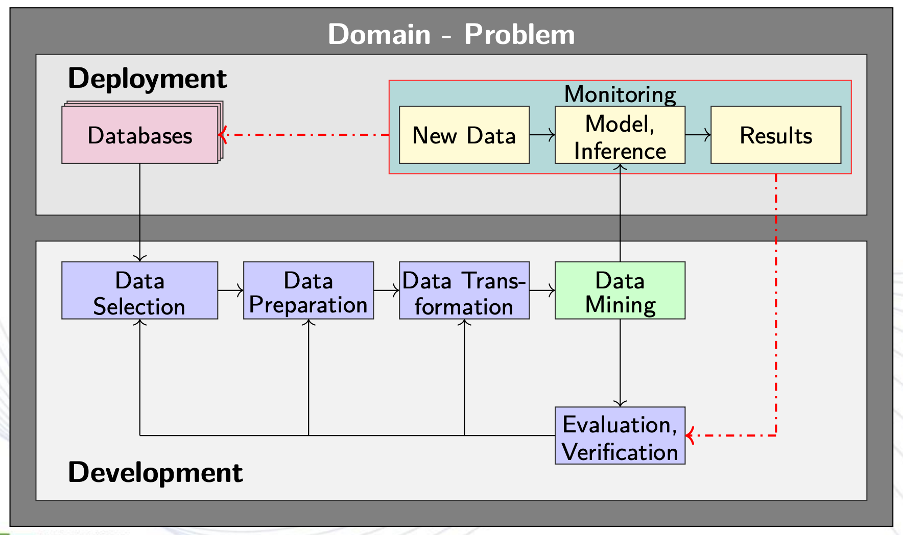
\includegraphics[height=90mm, width=130mm]{Images/KDDProcess}
		\end{center}
	\caption{ KDD Process Workflow \cite{Wings:2023}}
	\end{figure}
\end{center}

\ac{kdd} is the process of discovering useful information and knowledge from large data sets. It is an iterative process, where each stage may be revisited multiple times to refine the results and improve the accuracy of the analysis. It is a crucial procedure for drawing conclusions from huge data sets and has applications in a number of industries, including finance, healthcare, and business.\bigskip

KDD is the nontrivial process of identifying valid, novel, potentially useful, and ultimately understandable patterns in data\cite{fayyad:1996}. In order to predict future sales trends, detect patterns and trends in customer behaviour, and improve pricing and promotional methods, the KDD technique can be used. For businesses trying to increase the accuracy of their sales forecasting and make data-driven decisions, it is an essential method. It is extremely useful in the current technological world.\bigskip

And in this case, we're using KDD to recognise gestures, thus we must first lay out the aims and objectives of the experiment.The KDD technique is used to gather, develop, and anticipate the gesture as necessary after the goals have been specified.The complete procedure involves:\bigskip

\begin{itemize}
	\item \textbf{Data selection:}\smallskip

	The data that will be used for analysis are chosen during this stage. The information may originate from a number of places, including databases, data warehouses, and the internet.
 	\item \textbf{Preprocessing: }\smallskip 

	The data is cleaned, converted, and merged at this stage to get rid of any errors, inconsistencies, or missing values. In this phase, only the pertinent features that will be used for analysis are chosen during the feature selection process.
 	\item \textbf{Data transformation: }\smallskip 
	
	The data is changed into a format that will allow for analysis. This could involve aggregation, normalisation, or discretization.
 	\item \textbf{Data mining: }\smallskip 
 	
The updated data is analysed at this level using a variety of data mining techniques. These techniques include classification, clustering, association rule mining, and anomaly detection, to name a few.
 	\item \textbf{Evaluation: }\smallskip 
 	
	At this stage, the effectiveness and correctness of the data mining techniques' findings are assessed. This can entail applying cross-validation methods or testing the outcomes using a different data set.
 	\item \textbf{Interpretation: }\smallskip
  
	The final step is to interpret the results and generate insights into the sales prediction. This may involve creating reports or visualizations to communicate the results to stakeholders.
	
\end{itemize}

\section{Why KDD?}

For our project of sales forecasting, we chose KDD technique for the following reasons:

\begin{enumerate}
	\item \textbf{Data preprocessing:} In a sales forecasting problem, the dataset may contain missing values, outliers, and noisy data that can affect the accuracy of the regression model. KDD techniques such as data cleaning and data transformation can be used to preprocess the data and ensure that it is in a suitable format for analysis. For example, missing values can be imputed using techniques such as mean imputation, regression imputation, or k-nearest neighbors imputation. Outliers can be detected using methods such as z-score or interquartile range, and either removed or transformed using techniques such as winsorization or log transformation. Noisy data can be detected and corrected using methods such as filtering, smoothing, or clustering.

	\item \textbf{Feature selection:} In a sales forecasting problem, the dataset may contain a large number of features or variables that may not all be relevant for predicting sales. KDD techniques can be used to identify the most important features or variables to use in the regression model. For example, feature selection methods such as correlation analysis, forward selection, backward elimination, or lasso regression can be used to select the most relevant features. This can improve the accuracy and efficiency of the model, as it focuses only on the most important predictors.

	\item \textbf{Model selection and optimization:} In a sales forecasting problem, there are several regression algorithms that can be used, such as linear regression, logistic regression, ridge regression, or random forest regression. KDD techniques can be used to select the most appropriate algorithm and optimize its parameters to achieve the best performance  \cite{Azevedo:2008}. For example, cross-validation can be used to evaluate different models and compare their performance on the dataset. Hyperparameter tuning can be used to optimize the parameters of the selected model using techniques such as grid search or random search. This can help improve the accuracy and efficiency of the model.

	\item \textbf{Interpretation and visualization:} In a sales forecasting problem, it is important to interpret the results of the regression model and visualize the patterns and trends in the data. KDD techniques can be used to interpret the coefficients of the regression model and identify the factors that influence sales. For example, a coefficient of 0.5 for a feature indicates that a one-unit increase in that feature results in a 0.5-unit increase in sales. Visualization techniques such as scatter plots, line charts, or heatmaps can be used to visualize the patterns and trends in the data, and identify correlations or patterns that may be useful for sales forecasting. \cite{fayyad:1996}
	
\end{enumerate}	

In summary, KDD techniques can be applied in a sales forecasting problem using regression algorithms to preprocess the data, select relevant features, select an appropriate regression algorithm, optimize its parameters, and interpret and visualize the results. This can help improve the accuracy, efficiency, and interpretability of the sales forecasting model, and provide valuable insights and knowledge to support decision-making in sales and marketing.




